\documentclass{beamer}
\usepackage[utf8]{inputenc}
\usepackage{listings}
\usepackage{booktabs}
\usepackage{amssymb}
\usepackage{nicefrac}
\usepackage{amsmath}
\usepackage{bbm}
\usepackage{bm}
\usepackage{enumitem}
\usepackage{hyperref}
\usepackage[export]{adjustbox}
\usepackage{svg}

\usetheme{Madrid}
\definecolor{mlpblue}{rgb}{0.1, 0.14, 0.24}

\useoutertheme{infolines} % Alternatively: miniframes, infolines, split
\useinnertheme{circles}
\usecolortheme[named=mlpblue]{structure}

\DeclareMathOperator{\Tr}{Tr}
\DeclareMathOperator{\Cov}{Cov}
\DeclareMathOperator{\Concat}{Concat}

\DeclareMathOperator*{\argmax}{arg\,max}
\DeclareMathOperator*{\argmin}{arg\,min}
\DeclareMathOperator*{\indep}{\perp \!\!\! \perp}

\lstset{basicstyle=\footnotesize\ttfamily,breaklines=true}

%------------------------------------------------------------
%This block of code defines the information to appear in the
%Title page
\title[RoPE]{Rotational Positional Encoding}

\subtitle{RoPE} %\thanks{Beaglehole, Súkeník et.~al.~[NeurIPS 2024]}}
\author[MLP]{A. Buynitsky} 
\date{Jan 28, 2025}
\titlegraphic{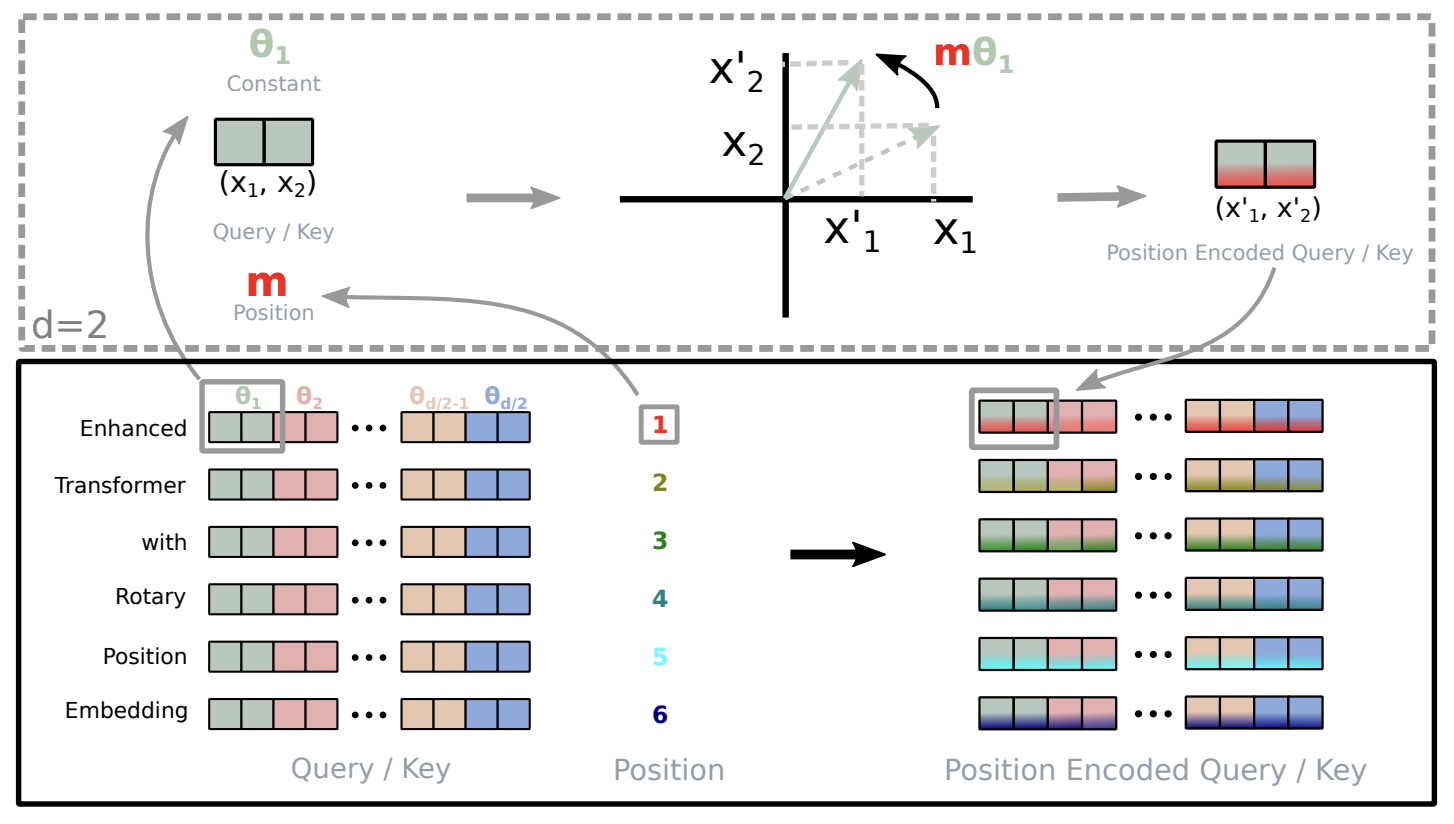
\includegraphics[width=6.5cm]{./img/title.png}}

%End of title page configuration block
%------------------------------------------------------------

%The next block of commands puts the table of contents at the 
%beginning of each section and highlights the current section:

\AtBeginSection[]
{
  \begin{frame}
    \frametitle{Outline}
    \tableofcontents[currentsection]
  \end{frame}
}
% ------------------------------------------------------------


\begin{document}

\frame{\titlepage}


%---------------------------------------------------------
% This block of code is for the table of contents after
% the title page
\begin{frame}
\frametitle{Outline}
\tableofcontents
\end{frame}
%---------------------------------------------------------
\section{Complex Numbers}
\begin{frame}[t]{What is a Complex Number}
    Define $i = \sqrt{-1}$ so $i^2 = -1$ \newline
    Any complex number $z = a + b i$ can be split into its real part:
    \[\text{Re}(Z) = a\]
    And imaginary part: 
    \[\text{Im}(z) = b\]
    \textbf{Example}: Find Re and Im parts of $(3 + 4i)(2 + 3i)$: \newline
    \begin{align*}
        (3 + 4i)(2 + 3i) &= 6 + 8i + 9i + 12(i^2)\\
        &= 6 + 8i + 9i - 12\\
        &= -6 + 17i
    \end{align*}





\end{frame}

\begin{frame}[t]{Euler's Formula}
    \begin{columns}
        \hspace{0.5em}
		\begin{column}{.6\textwidth}
            Consider the power series expansion of $e^z$: \newline
            \vspace{-1.8em}
            \begin{align*}
                e^z &= 1 + z + \frac{z^2}{2!} + \frac{z^3}{3!} + \frac{z^4}{4!} + \dots \\
                e^{iz}&= 1 + iz + \frac{(iz)^2}{2!} + \frac{(iz)^3}{3!} + \frac{(iz)^4}{4!} + \dots \\
                &= 1 + iz - \frac{(z)^2}{2!} - \frac{i z^3}{3!} + \frac{iz^4}{4!} + \dots \\
                &= (1 - \frac{z^2}{2!} + \frac{iz^4}{4!} + \dots) + (iz - \frac{i z^3}{3!} + \dots)\\
                &= (1 - \frac{z^2}{2!} + \frac{z^4}{4!} + \dots) + (iz - \frac{i z^3}{3!} + \dots)\\
                &= cos(z) + i sin(z)
            \end{align*}
            Therefore:
            \[r e^{i \theta} = r (cos(\theta) + i sin(\theta))\]
		\end{column}
        \hspace{0em}
		\begin{column}{.4\textwidth}
            \begin{center}
                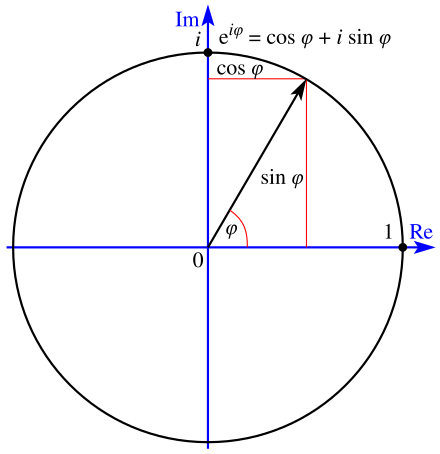
\includegraphics[width=0.9\textwidth]{./img/euler.png}
            \end{center}
		\end{column}
        \hspace{2em}
	\end{columns}
\end{frame}


\begin{frame}[t]{Representation and Properties of Complex Numbers}
    \begin{columns}
        \hspace{0.5em}
		\begin{column}{.7\textwidth}
            For a complex number $z$:
            \[z = r e^{i \theta} = r(cos\theta + sin \theta) = a + b i\]
            \textbf{Maginitude of Complex Number:}
            \[|z| = r = \sqrt{a^2 + b^2}\]
            \textbf{Argument (angle) of Complex Number:}
            \[\text{Arg} z = \theta = arctan(\frac{b}{a}) \text{ for } -\pi \leq \theta < \pi\]
            \[\text{arg} z = \theta + 2 \pi k  = arctan(\frac{b}{a}) + 2 \pi k \text{ for k } \in \mathbb{Z}\]
            \textbf{Conjugate of Complex Number:}
            \[ \overline{z} = r e ^{-i \theta} = r(cos \theta - sin\theta)\]
		\end{column}
        \hspace{0em}
		\begin{column}{.3\textwidth}
            \begin{center}
                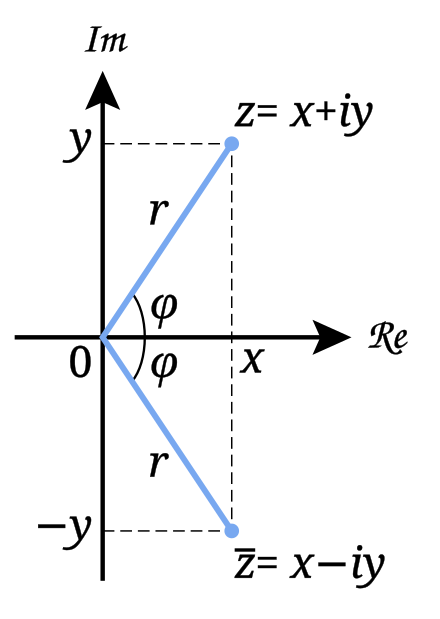
\includegraphics[width=1.0\textwidth]{./img/complex_conjugate.png}
            \end{center}
		\end{column}
        \hspace{2em}
	\end{columns}
\end{frame}

\section{Transformers}
\begin{frame}[t]{Transformers (part 1)}
    Define a sequence of input tokens and corresponding word embeddings:
    \begin{align*}
    \mathbb{S}_N &= \left\{w_i \right\}_{i=1}^N\\
    \mathbb{E}_N &= \left\{x_i \right\}_{i=1}^N
    \end{align*}
    where $x_i \in \mathbb{R}^d$ is embedding vector of token $w_i$ \textbf{without positional info}:
    \newline
    \textbf{Self Attention:}

    % encode two characteristics tokens:
    %1. tokens that are similar/related should have higher scores
    %2. score should be higher for words that are closer together
    Calculates: $q_m = f_q(x_m, m), k_n = f_k(x_n, n), v_n = f_v(x_n, n)$ with:
    \begin{gather}\label{eq:4}
        f_{t:t\in \left\{q,k,v\right\}} = \textbf{W}_{t:t\in \left\{q,k,v\right\}}(x_i + p_i)
    \end{gather}
    where $p_i$ is:
    \[
        \begin{cases}
        \begin{aligned}
        p_{2t} & = \sin\left(\frac{k}{10000} \cdot \frac{2t}{d}\right), \\
        p_{2t+1} & = \cos\left(\frac{k}{10000} \cdot \frac{2t}{d}\right).
        \end{aligned}
        \end{cases}
    \]
\end{frame}

\begin{frame}[t]{Attention}
    Calculate attention score and normalize with softmax: % normalize via softmax
    \[
        a_{m,n} =
        \frac{\exp\left(\frac{\mathbf{q}_m^\top \mathbf{k}_n}{\sqrt{d}}\right)}
        {\sum_{j=1}^N \exp\left(\frac{\mathbf{q}_m^\top \mathbf{k}_j}{\sqrt{d}}\right)}
    \]
    % keep intact values with words want to focus on, draw out irrelevant words and sum up weighted value vectors
    Extract values 
    \[o_m = \sum_{n=1}^N a_{m,n} v_n \]
\end{frame}

\section{Issue with Positional Encoding}
\begin{frame}[t]{Issue with positional encodings}
    % tokens that have similar embeddigns should have higher score
    % toekns that are close to each other should have higher score
    Let's consider a 2D case:
    \begin{itemize}[label=-]
        % think of dot product as magnitude and angle
        % when multiple k,q matrices, each square shows the weight to place on the value between word at n, word at m
        \item Similar tokens should have higher score $||q_m|| \cdot ||k_n||$ (magnitude) 
        % further apart words are, less likely for them to be related
        \item Closer tokens should have higher score $\Theta_{(m-n)}$
    \end{itemize}
    \begin{center}
        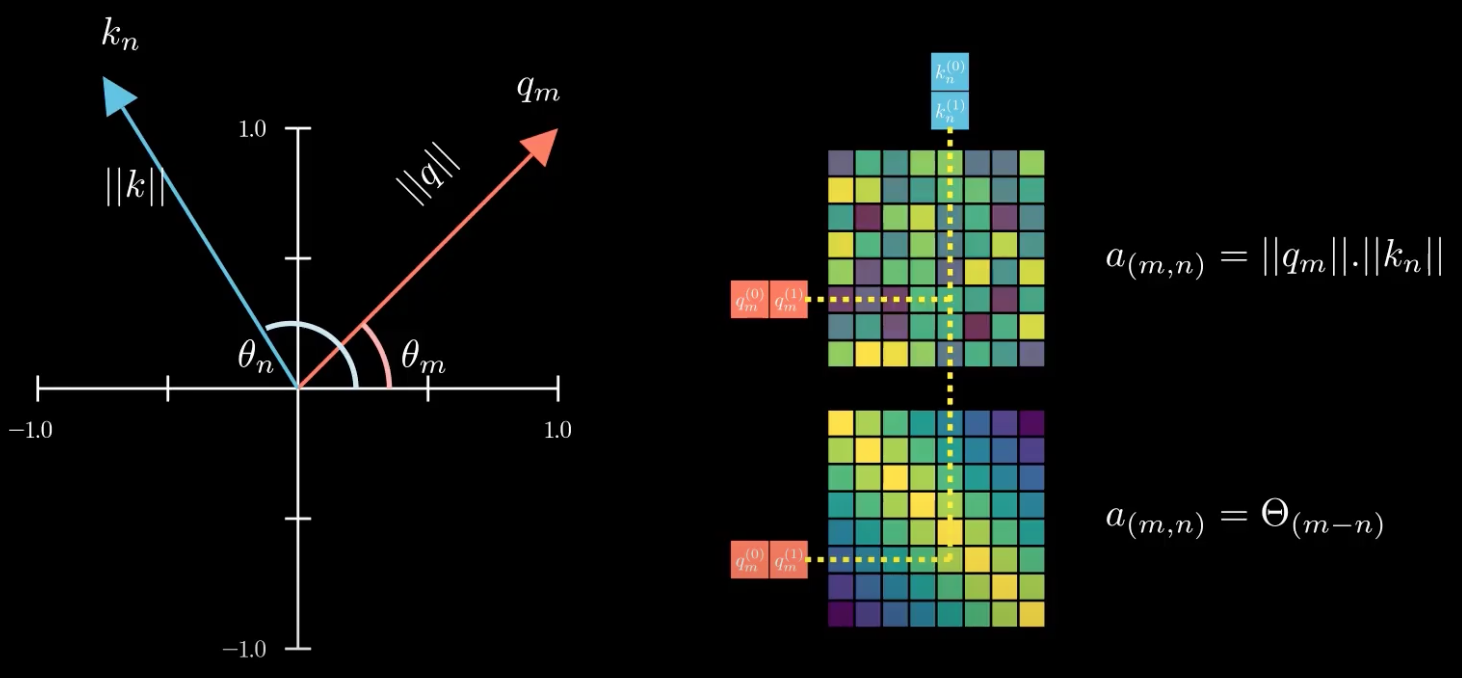
\includegraphics[width=0.9\textwidth]{./img/rope_1.png}
    \end{center}
    \small Shoutout to https://www.youtube.com/watch?v=GQPOtyITy54 for visuals
    \normalsize
\end{frame}
\begin{frame}[t]{Issue with positional encodings (cont)}
    % tokens that have similar embeddigns should have higher score
    % toekns that are close to each other should have higher score
    Let's consider a 2D case:
    \begin{itemize}[label=-]
        % think of dot product as magnitude and angle
        % when multiple k,q matrices, each square shows the weight to place on the value between word at n, word at m
        \item Similar tokens should have higher score $||q_m|| \cdot ||k_n||$ (magnitude) 
        % further apart words are, less likely for them to be related
        \item Closer tokens should have higher score $\Theta_{(m-n)}$
    \end{itemize}
    \begin{center}
        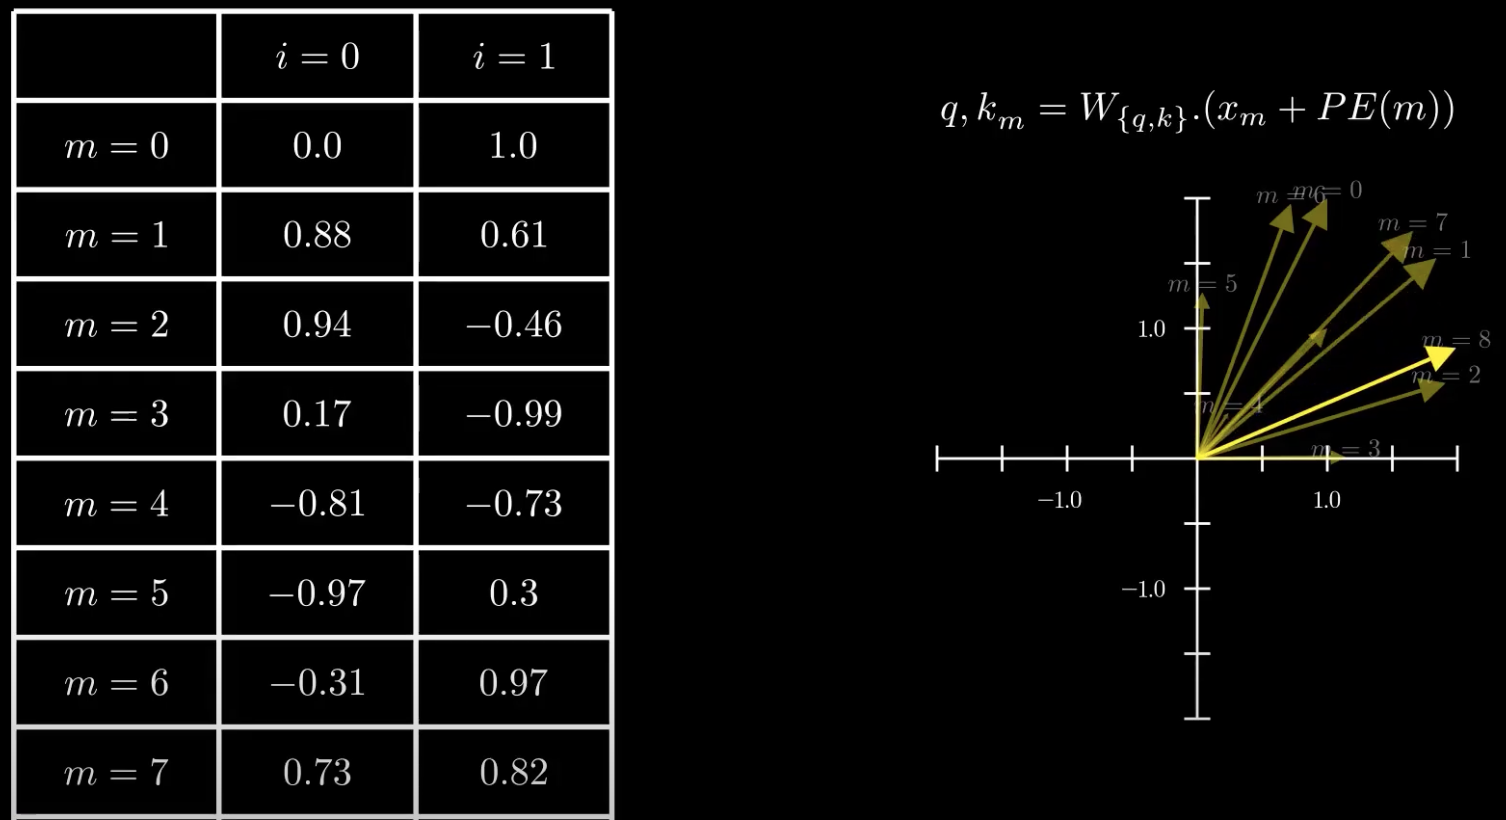
\includegraphics[width=0.8\textwidth]{./img/rope_2.png}
    \end{center}
    Problem: Combined positional and token embeddings together
\end{frame}
\section{Derivation}
\begin{frame}[t]{Reformulation}
    For each inner product, we want: \[q_m^T k_n = \langle f_q(x_m, m), f_k(x_n, n) \rangle = g(x_m, x_n, m - n)\]
    In 2D case, convert vectors to complex numbers:
    \begin{align}
        q_m &= R_q(x_m, m)e^{i \Theta_q(x_m,m)} \\
        k_n &= R_k(x_n, n)e^{i \Theta_k(x_n,n)} \\
        g(x_m, x_n, n - m) &= R_g(x_m, x_n, n - m) e^{i \Theta_g(x_m, x_n, n - m)}\\
        q_m^T &= R_q(x_m, m)e^{-i \Theta_q(x_m,m)}
    \end{align}
    Multiply $q_m^T \cdot k_n$ in complex numbers:
    \begin{align}
        q_m^T \cdot k_n = R_q(x_m, m) \cdot R_k(x_n, n) e^{i (\Theta_k(x_n,n) - \Theta_q(x_m,m))}
    \end{align}
    % solve and get the follwoing two equations:
    % m - n represents relative position info between two vectors
    % when take transpose, same as taking complex conjugate
\end{frame}

\begin{frame}[t]{Determine Magintude}
    \vspace{-3em}
    \begin{gather}\label{eq:mag}
        R_q(x_m, m) R_k(x_n, n) = R_g(x_m, x_n, n - m)
    \end{gather}
    \vspace{-3em}
    \begin{gather}\label{eq:arg}
        \Theta_k(x_n, n) - \Theta_q(x_m, m) = \Theta_g(x_m, x_n, n - m)
    \end{gather}
    % will mean that equ 12 will go to 0 
    Now suppose that $m = n$. Then left with just \ref{eq:mag} \newline
    \[R_q(x_m, m) R_k(x_n, n) = R_g(x_m, x_n, 0)\]
    Now set $m = n = 0$
    \[R_g(x_m, x_n, 0) = R_q(x_m, 0) R_k(x_n, 0) = ||q|| \; ||k ||\]
    Therefore:
    \[R_q(x_m, m) = ||q|| \text{ and } R_k(x_n, n) = || k ||\]
\end{frame}

\begin{frame}[t]{Determine Argument}
    By a similar trick setting $m=n$:
    \begin{align}
        \Theta_q(x_m, m) - \Theta(x_n, n) &= \Theta_g(x_m, x_n, 0)\\
        &= \Theta(x_m, 0) - \Theta(x_n, 0) = \theta_q - \theta_k
    \end{align}
    Rearranging, we get:
    \[\Theta_q(x_m, m) - \theta_q = \Theta_k(x_n, m) - \theta_k\]
    Observe that values only related to $m$, independent if $x = x_n$ or $x = x_m$ \newline
    Let $\phi(m)$ to be:
    % can take either side of the equation
    \[\phi(m) = \Theta_q(x_m, m) - \theta_q = \Theta_k(x_n, n) - \theta_k\]
\end{frame}

\begin{frame}[t]{Determine Argument}
    Recall:
    \[\Theta_q(x_m, m) - \Theta_k(x_n, n) = \Theta_g(x_m, x_n, n-m)\]
    and let $n = m+1$ so:
    \begin{gather}\label{eq:subst}
    \Theta_q(x_m, m) - \Theta_k(x_{m+1}, m+1) = \Theta_g(x_m, x_{m+1}, 1)
    \end{gather}
    Now:
    \begin{align*}
       \phi(m) &= \Theta_q(x_m, m) - \theta_q \Longrightarrow \Theta_q(x_m,m) = \phi(m) + \theta_q\\ 
       \phi(m+1)&= \Theta_k(x_{m+1}, m+1) - \theta_k \Longrightarrow \Theta_k(x_{m+1}, m+1) = \phi(m+1) + \theta_k
    \end{align*}
    Plugging into \ref{eq:subst}:
    \begin{align*}
        \phi(m) + \theta_q - (\phi(m+1) + \theta_k) &= \Theta_g(x_m, x_{m+1}, 1) \\
        \phi(m) - \phi(m+1) &= \Theta_g(x_m, x_{m+1}, 1)  - \theta_q + \theta_k
    \end{align*}
    RHS is constant irrelevant to $m$! $\phi(m)$ has constant difference between term regardless of $m$ so its an arithmetic sequence!\newline
    \vspace{-1em}
    \[\phi(m) = m \theta + \gamma\]
\end{frame}

\begin{frame}[t]{Combining Everything}
    \vspace{-2.5em}
    \begin{align}
        % q is q_m 
        q_m = f_q(x_m, m) &= R_q(x_m, m) e^{i \Theta_q (x_m, m)}\\
                          &= ||q|| e^{i \Theta_q (x_m, m)}\\
                          &= ||q|| e^{i (\phi(m) + \theta_q)}\\
                          &= ||q|| e^{i (m \theta + \gamma + \theta_q)}\\
                          &= ||q|| e^{i \theta_q}e^{i (m \theta + \gamma)}\\
                          &= q e^{i (m \theta + \gamma)}
    \end{align}
    Recall that:
    \[q_m = f_q(x_m, m) = W_q(x_m + p_m)\]
    so if $p_m = 0$, then
    \[ q_m = W_q \cdot x_m\]
    Therefore assume no position info when $m=0$ so let $\gamma = 0$.\newline
    % do not rotate the input
    % cool thing get is roots of unity
    \textbf{Final Result:}
    \[ f_q(x_m, m) = (W_q x_m)e^{i m \theta}\]
    \[ f_k(x_n, n) = (W_k x_n)e^{i n \theta}\]

\end{frame}

\begin{frame}[t]{Matrix Equations}
    Matrix form of equations in 2D
    \begin{center}
        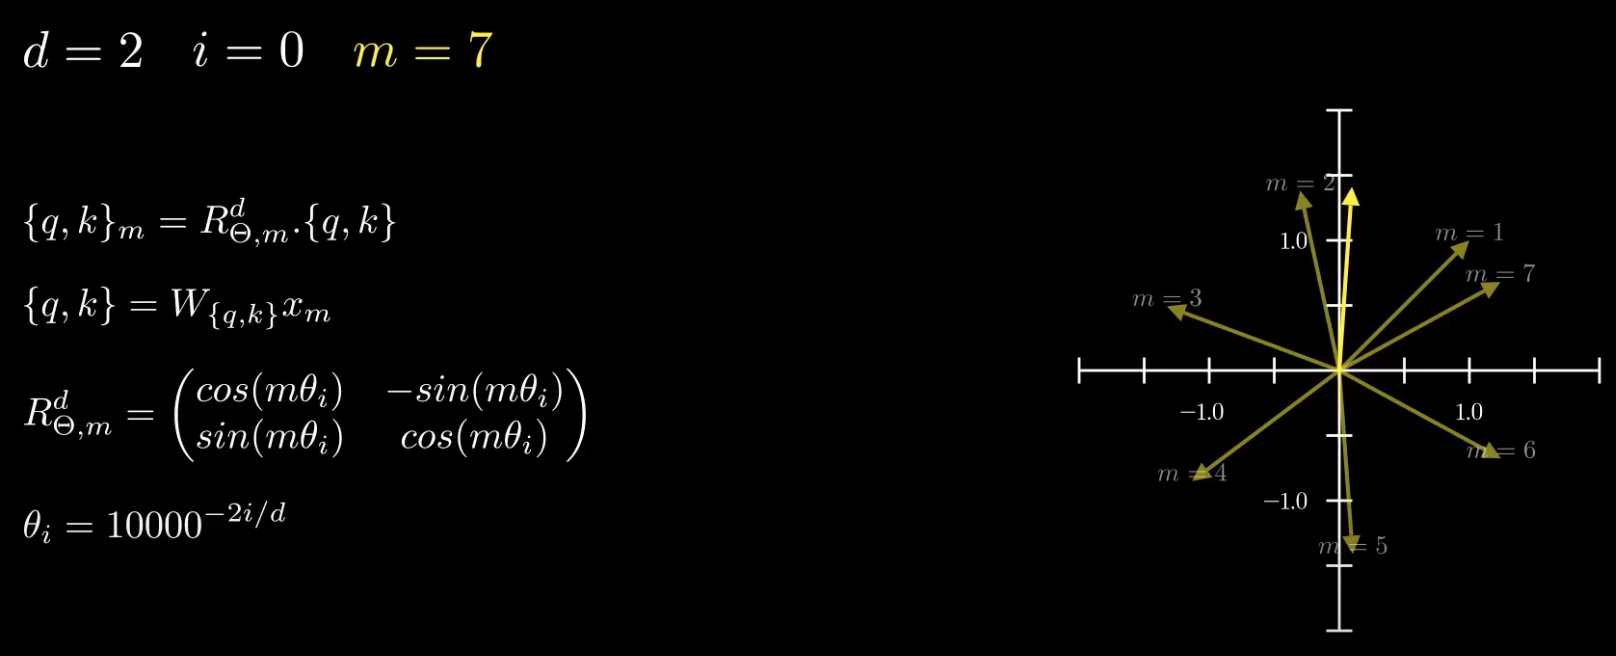
\includegraphics[width=1.0\textwidth]{./img/rope_3.png}
    \end{center}
\end{frame}

\begin{frame}[t]{Extending beyond d=2}
    Extending to multiple dimensions
    % break q and k d dimensional in d/2 blocks will repeat for each block indep
    % convert to block diag rotational matrix, each rotation block have own constant
    % will depend on index across dimension
    \begin{center}
        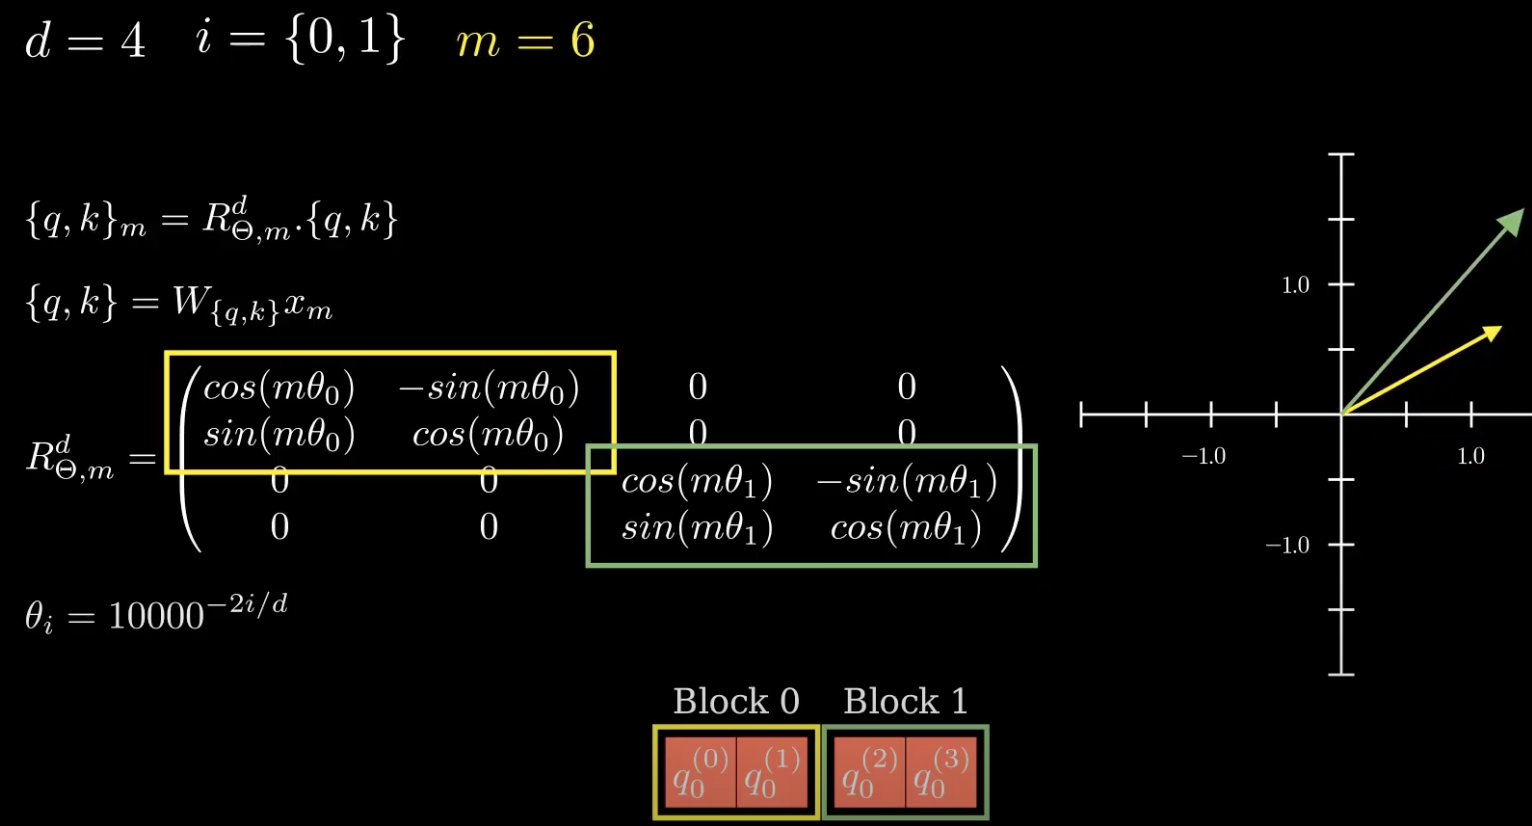
\includegraphics[width=1.0\textwidth]{./img/rope_4.png}
    \end{center}
\end{frame}

\section{Result}

\begin{frame}[t]{Result}
    Increases Sequence prediction confidence (perplexity):
    % perplexity measures how confused model is (think predicting 5 words with = probability)
    \begin{center}
        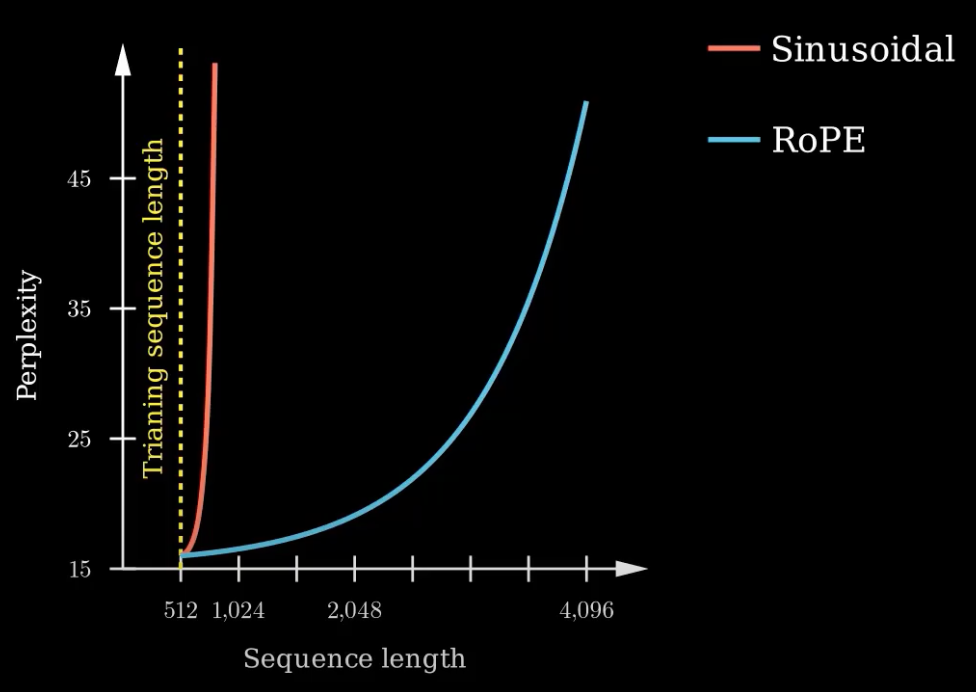
\includegraphics[width=0.8\textwidth]{./img/rope_5.png}
    \end{center}
\end{frame}

\begin{frame}{Thank you!}
	\begin{center}
        Have a great rest of your Day!!!
	\end{center}
	\begin{center}
		% \textbf{Slides:} {\small \url{https://cs.purdue.edu/homes/jsetpal/slides/dnc_by_agop.pdf}}
	\end{center}
\end{frame}


\end{document}